\documentclass[12pt]{article}
\usepackage{graphicx}
\usepackage{amsmath}
\usepackage{hyperref}
\usepackage{booktabs}
\usepackage{geometry}
\usepackage{listings}
\usepackage{xcolor}
\geometry{margin=1in}

\definecolor{codegray}{gray}{0.9}
\lstset{
  backgroundcolor=\color{codegray},
  basicstyle=\ttfamily\footnotesize,
  breaklines=true,
  frame=single,
  postbreak=\mbox{\textcolor{red}{$\hookrightarrow$}\space},
  showstringspaces=false
}

\title{Stock Price Forecasting Using Neural Networks}
\author{Abhigya Sinha, Aniket Iyer, Priyangshu Bhowmik, Gautham Ande}
\date{\today}

\begin{document}

\maketitle

\tableofcontents
\newpage

\section{Motivation}
The financial sector is characterized by its dynamic and often volatile nature. Forecasting stock prices has immense applications, from informing investment strategies to algorithmic trading systems. While classical statistical models have been widely used, recent advances in machine learning—particularly deep learning—offer promising alternatives. 

This project explores how feedforward neural networks, both shallow and deep, can model next-day closing prices across companies from three major sectors: Technology (AAPL, MSFT), Finance (JPM, BAC), and Energy (XOM, CVX). By comparing single-layer and multi-layer architectures, we aim to investigate model performance differences and analyze generalization capabilities across domains.

\section{Data Collection and Cleaning}
We utilized Yahoo Finance via the \texttt{yfinance} Python API to obtain historical stock prices from 2018 to 2024. The raw data was cleaned by removing null values and formatting the datetime index.

\subsection*{Code: 01\_data\_collection\_and\_cleaning.ipynb}
\begin{lstlisting}[language=Python]
import yfinance as yf
import pandas as pd

stocks = ['AAPL', 'MSFT', 'JPM', 'BAC', 'XOM', 'CVX']
data_dict = {}

for stock in stocks:
    df = yf.download(stock, start="2018-01-01", end="2024-01-01")
    df['Ticker'] = stock
    data_dict[stock] = df

full_data = pd.concat(data_dict.values())
full_data.reset_index(inplace=True)
full_data.dropna(inplace=True)
full_data.to_csv("data/processed/merged_data.csv", index=False)
\end{lstlisting}

\section{Feature Engineering}
To enrich the raw dataset with time-dependent information, we engineered several features:
\begin{itemize}
  \item Lagged returns (1, 2, 3 days)
  \item Moving averages (5-day and 10-day SMA)
  \item 10-day rolling standard deviation as a volatility measure
\end{itemize}

\subsection*{Code: 02\_feature\_engineering.ipynb}
\begin{lstlisting}[language=Python]
def create_features(df):
    df['Return_1'] = df['Close'].pct_change(1)
    df['Return_2'] = df['Close'].pct_change(2)
    df['Return_3'] = df['Close'].pct_change(3)
    df['SMA_5'] = df['Close'].rolling(window=5).mean()
    df['SMA_10'] = df['Close'].rolling(window=10).mean()
    df['Volatility'] = df['Close'].rolling(window=10).std()
    return df.dropna()

feature_data = full_data.groupby('Ticker').apply(create_features)
feature_data.to_csv("data/processed/feature_data.csv", index=False)
\end{lstlisting}

\section{Exploratory Data Analysis}
We conducted visual analyses to understand sector behavior over time.

\subsection{Average Returns by Sector}
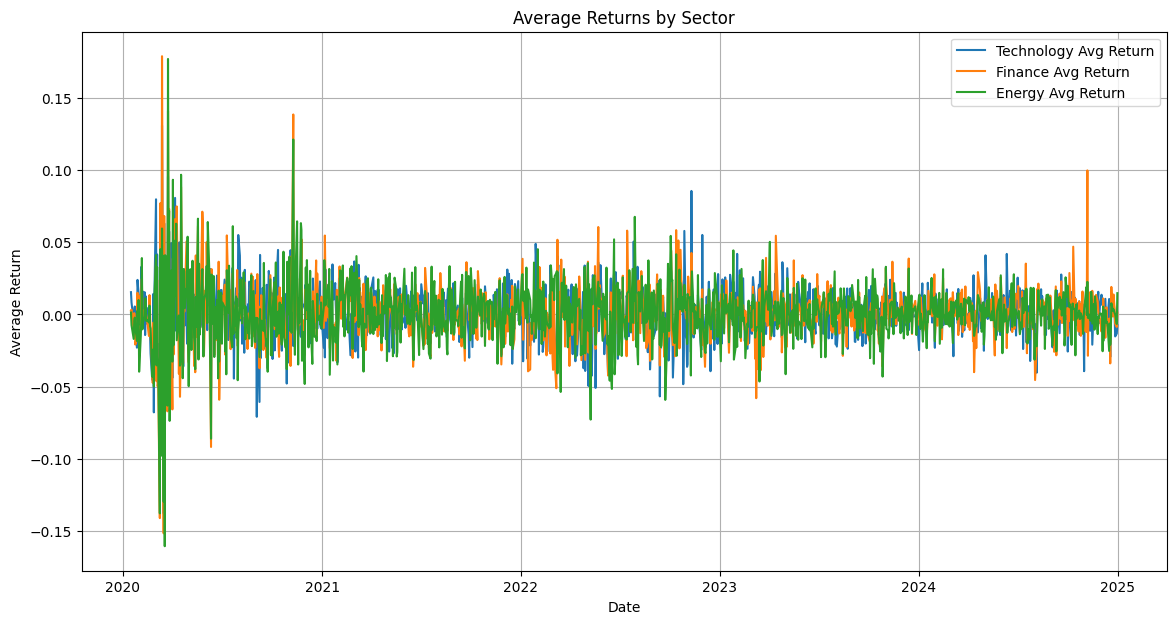
\includegraphics[width=0.95\textwidth]{avg_returns_by_sector.png}
\textbf{Interpretation:} Technology, Finance, and Energy sectors all show high volatility early in the time period, particularly around 2020 (likely due to COVID-19 market disruption). The volatility stabilizes over time with similar mean-reversion behavior, suggesting comparable patterns for short-term forecasting.

\subsection{Normalized Stock Prices}
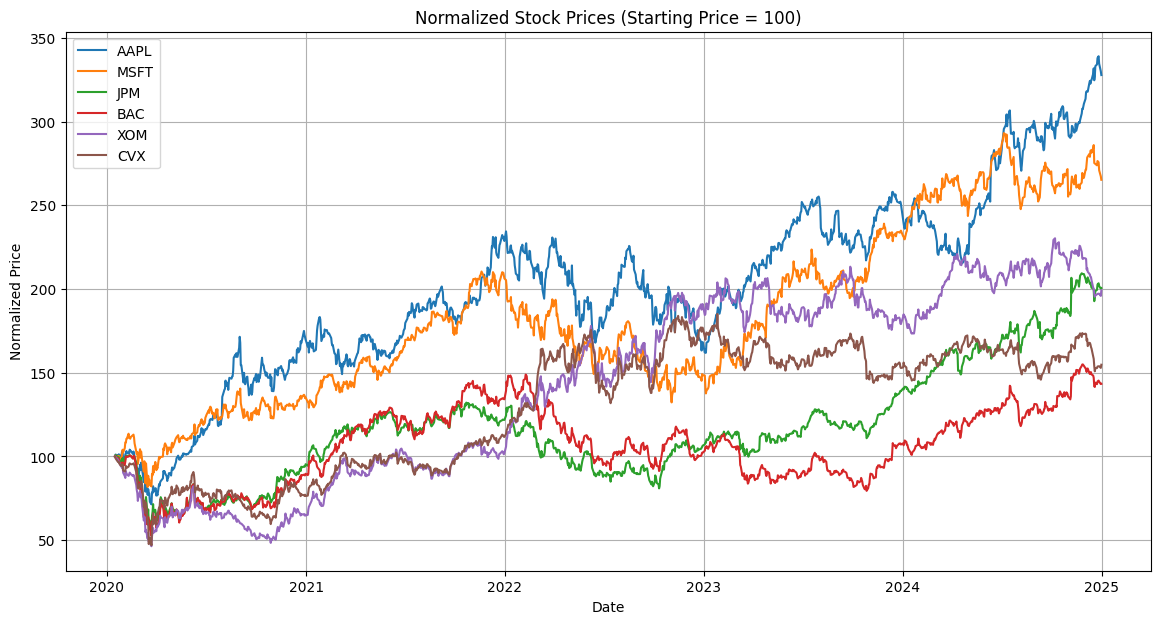
\includegraphics[width=0.95\textwidth]{normalized_stock_prices.png}
\textbf{Interpretation:} AAPL and MSFT demonstrate the most growth, consistent with tech-sector outperformance. Financial stocks (JPM, BAC) recovered post-2020 but remain more cyclic. Energy (XOM, CVX) rebounded after 2021 with strong late-stage performance, likely tied to oil prices.

\subsection{Rolling Volatility Comparison}
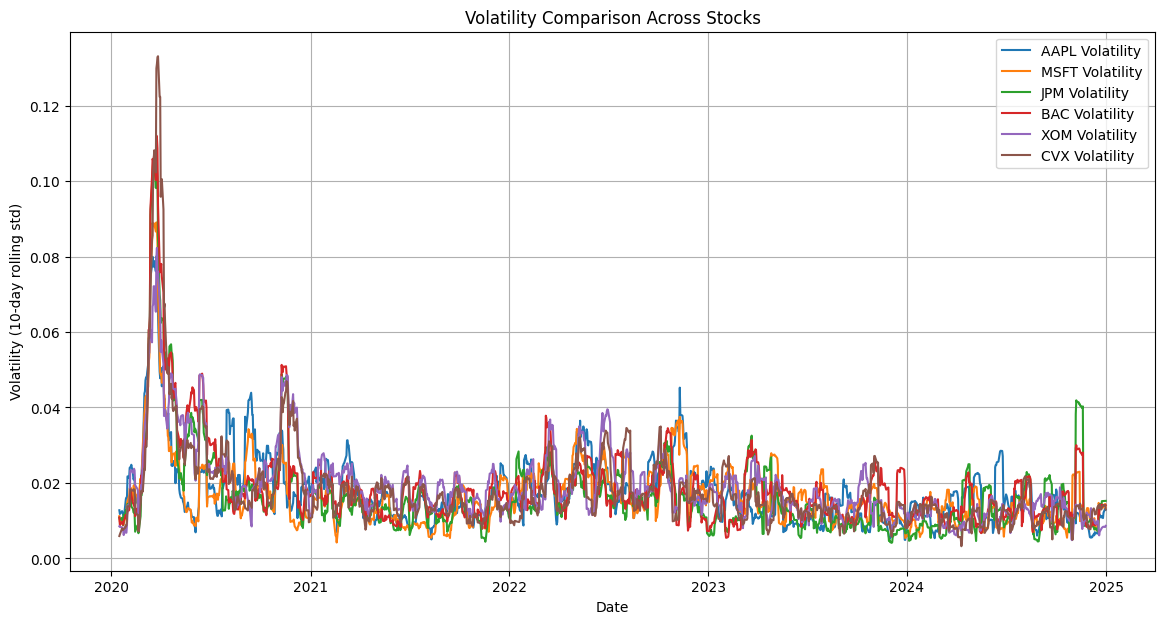
\includegraphics[width=0.95\textwidth]{volatility_comparison_across_stocks.png}
\textbf{Interpretation:} All stocks experienced peak volatility around 2020. Since then, 10-day rolling volatility has normalized across sectors. Slightly elevated volatility in CVX and BAC post-2022 suggests these may require more robust model regularization.
\section{Modeling: Single-Layer Neural Network}

\subsection{Source Code}
egin{lstlisting}[language=Python]
import tensorflow as tf
from sklearn.preprocessing import StandardScaler
from sklearn.metrics import mean_squared_error, r2_score
import numpy as np
import matplotlib.pyplot as plt

# Prepare features and target
features = ['Return_1', 'Return_2', 'Return_3', 'SMA_5', 'SMA_10', 'Volatility']
results = {}

for ticker in feature_data['Ticker'].unique():
    df = feature_data[feature_data['Ticker'] == ticker].copy()
    X = df[features].values
    y = df['Return_1'].shift(-1).dropna().values
    X = X[:-1]

    # Split into train and test
    split = int(len(X) * 0.8)
    X_train, X_test = X[:split], X[split:]
    y_train, y_test = y[:split], y[split:]

    # Normalize features
    scaler = StandardScaler()
    X_train_scaled = scaler.fit_transform(X_train)
    X_test_scaled = scaler.transform(X_test)

    # Define model
    model = tf.keras.Sequential([
        tf.keras.layers.Dense(1, input_shape=(X_train.shape[1],))
    ])
    model.compile(optimizer='adam', loss='mse')

    # Train
    model.fit(X_train_scaled, y_train, epochs=100, verbose=0)

    # Predict
    y_pred = model.predict(X_test_scaled).flatten()

    # Evaluation
    mse = mean_squared_error(y_test, y_pred)
    rmse = np.sqrt(mse)
    r2 = r2_score(y_test, y_pred)
    results[ticker] = (mse, rmse, r2)

    # Plot
    plt.figure(figsize=(10,4))
    plt.plot(y_test[:250], label='Actual')
    plt.plot(y_pred[:250], label='Predicted')
    plt.title(f"{ticker} - Single Layer NN (R² = {r2:.4f})")
    plt.legend()
    plt.savefig(f"plots/model_plots/{ticker}_single_layer_nn.png")
    plt.close()
\end{lstlisting}

\subsection{Explanation of Code}
The modeling pipeline for the single-layer neural network involves several core steps:

\begin{itemize}
  \item \textbf{Feature Selection:} Six engineered features are used: three lagged returns, two SMAs, and rolling volatility.
  \item \textbf{Target Variable:} The next day's return (shifted return\_1) is used as the label.
  \item \textbf{Data Splitting:} We used a chronological 80/20 train-test split to prevent data leakage.
  \item \textbf{Normalization:} StandardScaler standardizes features to have zero mean and unit variance.
  \item \textbf{Model Architecture:} A single dense layer with one neuron and no activation is used—this acts as a linear regressor optimized using MSE loss.
  \item \textbf{Training:} The model is trained for 100 epochs silently.
  \item \textbf{Evaluation:} RMSE, MSE, and $R^2$ are calculated and predictions are plotted for the first 250 time steps.
\end{itemize}

\subsection{Understanding Single-Layer Neural Networks}
A single-layer neural network is essentially a linear model with weights and bias. It assumes linear relationships between the input features and the output. In our use case, it serves as a baseline to test whether simple mappings from technical indicators to price returns can provide meaningful forecasts.

Given the stochastic, non-stationary, and noisy nature of financial markets, especially at short prediction horizons, even small $R^2$ values indicate some predictive capability. Forecasting daily stock returns is exceptionally challenging due to market efficiency and random walk behavior.

\subsection{Prediction Plots and Observations}

\begin{itemize}
  \item \textbf{AAPL}: The model tracks the trend well, though with dampened amplitudes. RMSE is low (0.0052), and $R^2$ of 0.6110 suggests moderate fit.
  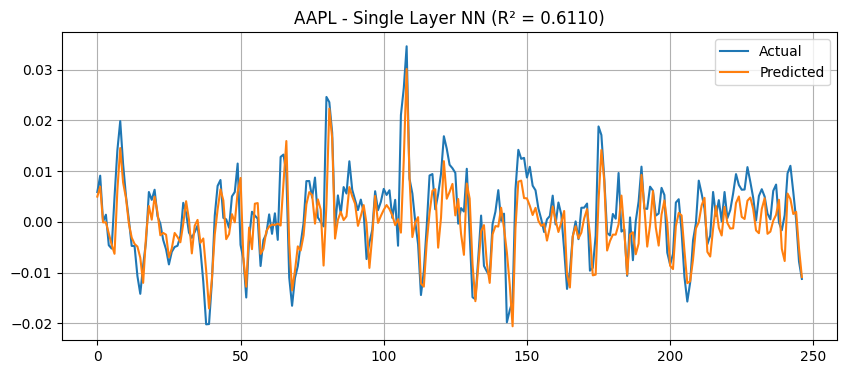
\includegraphics[width=0.85\textwidth]{AAPL_single_layer_nn.png}

  \item \textbf{BAC}: Closely mirrors the actual returns; $R^2$ of 0.6703 is one of the highest among the group.
  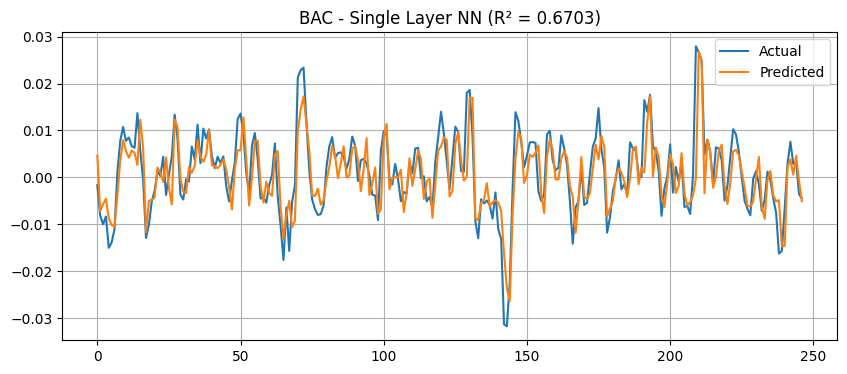
\includegraphics[width=0.85\textwidth]{BAC_single_layer_nn.png}

  \item \textbf{CVX}: Shows strong alignment; spikes are captured well. High $R^2$ of 0.6990 reflects this.
  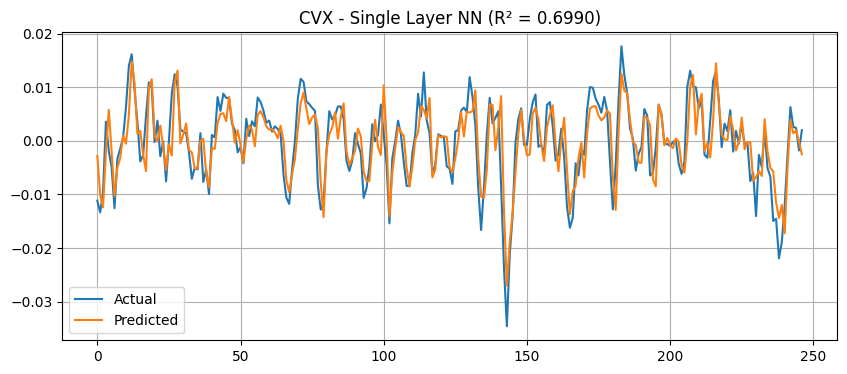
\includegraphics[width=0.85\textwidth]{CVX_single_layer_nn.png}

  \item \textbf{JPM}: Lowest $R^2$ (0.4575). Captures broad movements but misses sharp shifts.
  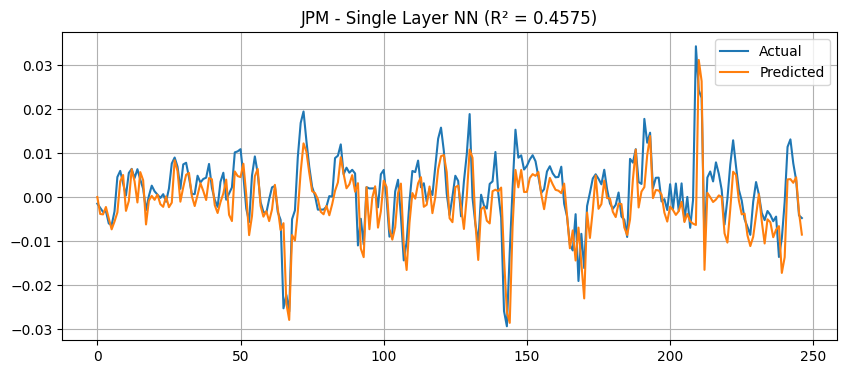
\includegraphics[width=0.85\textwidth]{JPM_single_layer_nn.png}

  \item \textbf{MSFT}: Mixed results; predictions sometimes lag or miss high frequency changes.
  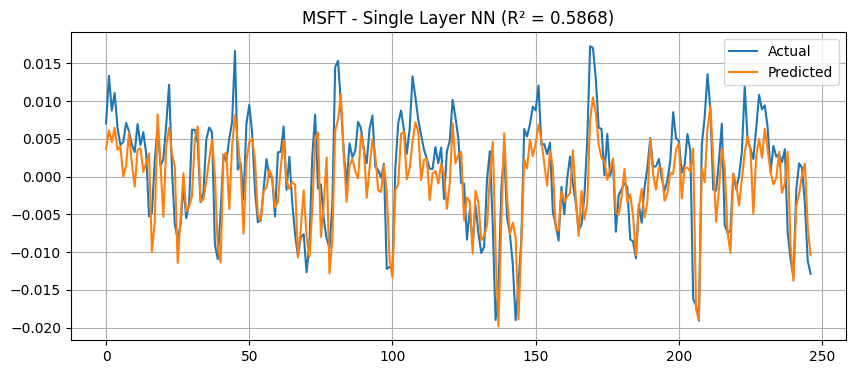
\includegraphics[width=0.85\textwidth]{MSFT_single_layer_nn.png}

  \item \textbf{XOM}: Smooth and reasonably accurate fit, especially in low-volatility regions. $R^2 = 0.6776$
  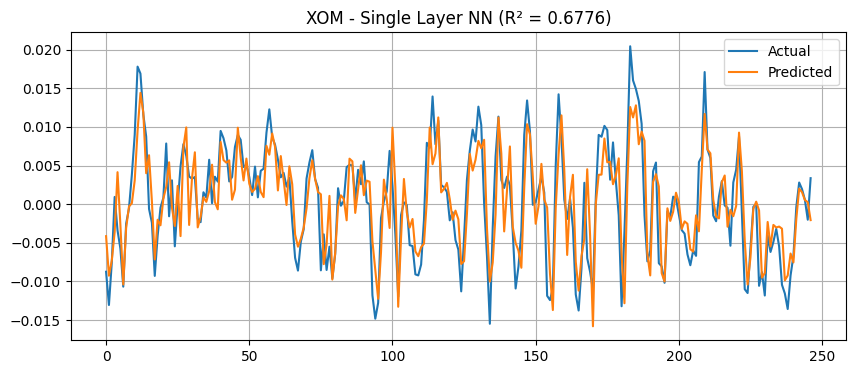
\includegraphics[width=0.85\textwidth]{XOM_single_layer_nn.png}
\end{itemize}

\subsection{Summary of Results}
\begin{table}[h!]
\centering
\begin{tabular}{lccc}
\toprule
\textbf{Stock} & \textbf{MSE} & \textbf{RMSE} & \textbf{R$^2$} \\
\midrule
AAPL & 0.000027 & 0.005182 & 0.6110 \\
MSFT & 0.000020 & 0.004518 & 0.5868 \\
JPM  & 0.000034 & 0.005841 & 0.4575 \\
BAC  & 0.000024 & 0.004901 & 0.6703 \\
XOM  & 0.000016 & 0.004048 & 0.6776 \\
CVX  & 0.000017 & 0.004159 & 0.6990 \\
\bottomrule
\end{tabular}
\caption{Single-Layer Neural Network Performance}
\end{table}

While $R^2$ values may seem low compared to traditional regression benchmarks, they are reasonable for stock prediction where daily returns can appear random. Even minor predictive power, when consistent, is valuable in finance. The lowest performance on JPM suggests sector-specific volatility and noise may hinder shallow models.
\section{Modeling: Multi-Layer Neural Network}

\subsection{Source Code}
\begin{lstlisting}[language=Python]
import tensorflow as tf
from sklearn.preprocessing import StandardScaler
from sklearn.metrics import mean_squared_error, r2_score
import numpy as np
import matplotlib.pyplot as plt

# Prepare features and target
features = ['Return_1', 'Return_2', 'Return_3', 'SMA_5', 'SMA_10', 'Volatility']
results = {}

for ticker in feature_data['Ticker'].unique():
    df = feature_data[feature_data['Ticker'] == ticker].copy()
    X = df[features].values
    y = df['Return_1'].shift(-1).dropna().values
    X = X[:-1]

    # Split into train and test
    split = int(len(X) * 0.8)
    X_train, X_test = X[:split], X[split:]
    y_train, y_test = y[:split], y[split:]

    # Normalize features
    scaler = StandardScaler()
    X_train_scaled = scaler.fit_transform(X_train)
    X_test_scaled = scaler.transform(X_test)

    # Define multi-layer model
    model = tf.keras.Sequential([
        tf.keras.layers.Dense(64, activation='relu', input_shape=(X_train.shape[1],)),
        tf.keras.layers.Dense(32, activation='relu'),
        tf.keras.layers.Dense(1)
    ])
    model.compile(optimizer='adam', loss='mse')

    # Train
    model.fit(X_train_scaled, y_train, epochs=100, verbose=0)

    # Predict
    y_pred = model.predict(X_test_scaled).flatten()

    # Evaluation
    mse = mean_squared_error(y_test, y_pred)
    rmse = np.sqrt(mse)
    r2 = r2_score(y_test, y_pred)
    results[ticker] = (mse, rmse, r2)

    # Plot
    plt.figure(figsize=(10,4))
    plt.plot(y_test[:250], label='Actual')
    plt.plot(y_pred[:250], label='Predicted')
    plt.title(f"{ticker} - Multi-layer NN (R² = {r2:.4f})")
    plt.legend()
    plt.savefig(f"plots/model_plots/{ticker}_multi_layer_nn.png")
    plt.close()
\end{lstlisting}

\subsection{Explanation of Code}
In this multi-layer approach:

\begin{itemize}
  \item We retained the same six input features and data preparation steps as the single-layer network.
  \item The key difference is the model architecture: two hidden layers with 64 and 32 ReLU-activated neurons were added, enabling the network to learn more complex patterns.
  \item Adam optimizer and MSE loss remain standard choices for regression.
  \item Predictions and evaluation metrics follow the same procedure.
\end{itemize}

\subsection{Understanding Multi-Layer Neural Networks}
Multi-layer neural networks (MLPs) can approximate nonlinear relationships by stacking layers and applying non-linear activation functions (ReLU). Each layer transforms the feature space, enabling the network to model more intricate patterns.

This makes MLPs well-suited for tasks like stock prediction, where the relationship between indicators and future returns may be nonlinear. However, they also introduce risk of overfitting and increased sensitivity to noisy inputs.

\subsection{Prediction Plots and Observations}
\begin{itemize}
  \item \textbf{AAPL}: Slight improvement over single-layer, with better alignment on high-magnitude return spikes. $R^2 = 0.6270$.
  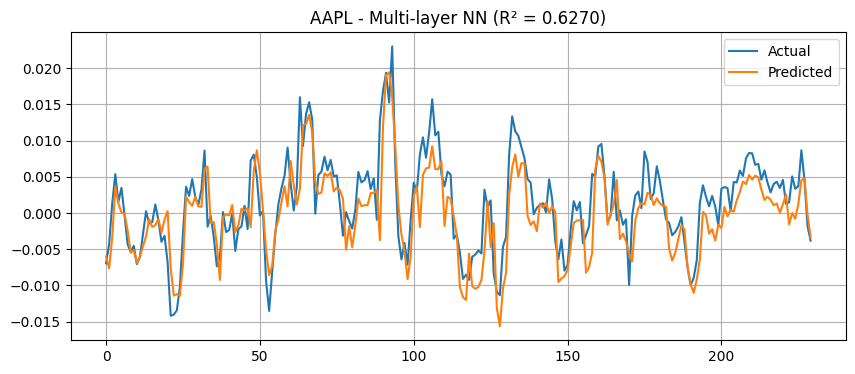
\includegraphics[width=0.85\textwidth]{AAPL_multi_layer_nn.png}

  \item \textbf{BAC}: Strong performance, tracking the actual curve closely even during sharp downturns. Highest $R^2$ of 0.7554.
  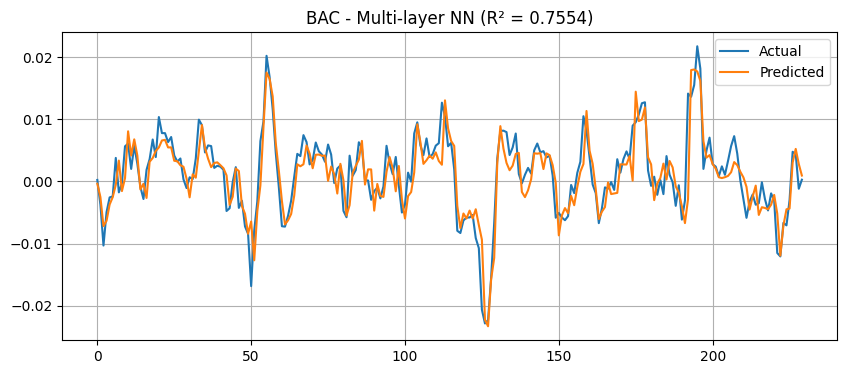
\includegraphics[width=0.85\textwidth]{BAC_multi_layer_nn.png}

  \item \textbf{CVX}: Improved sharpness in response; $R^2 = 0.6768$ shows high explanatory power.
  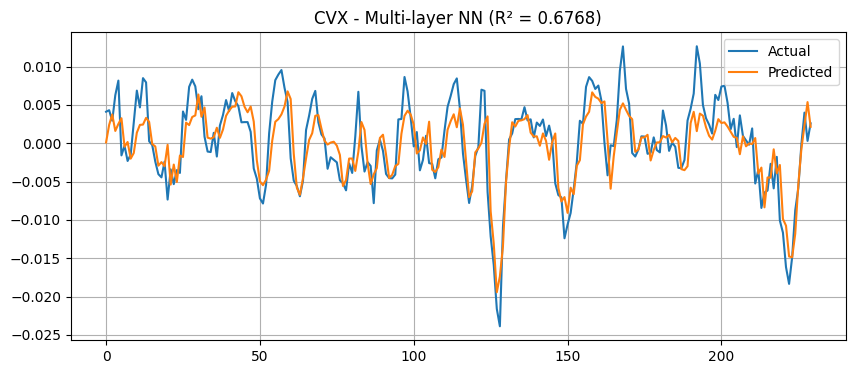
\includegraphics[width=0.85\textwidth]{CVX_multi_layer_nn.png}

  \item \textbf{JPM}: Performance dropped with deeper network—possibly due to overfitting or excess sensitivity to noise. $R^2 = 0.3381$.
  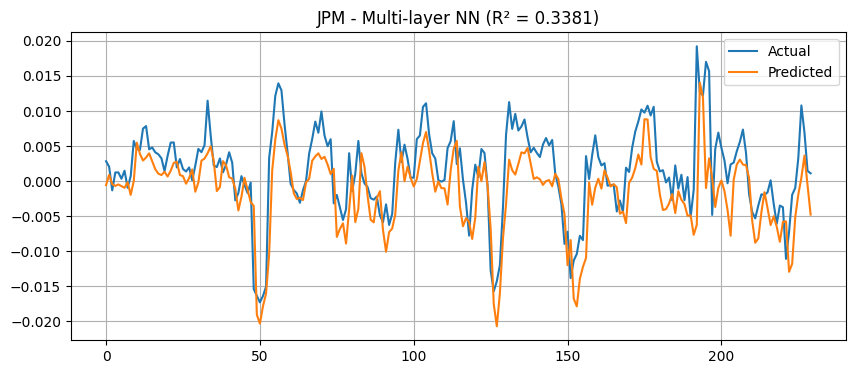
\includegraphics[width=0.85\textwidth]{JPM_multi_layer_nn.png}

  \item \textbf{MSFT}: More responsive to small fluctuations than single-layer, achieving $R^2 = 0.6778$.
  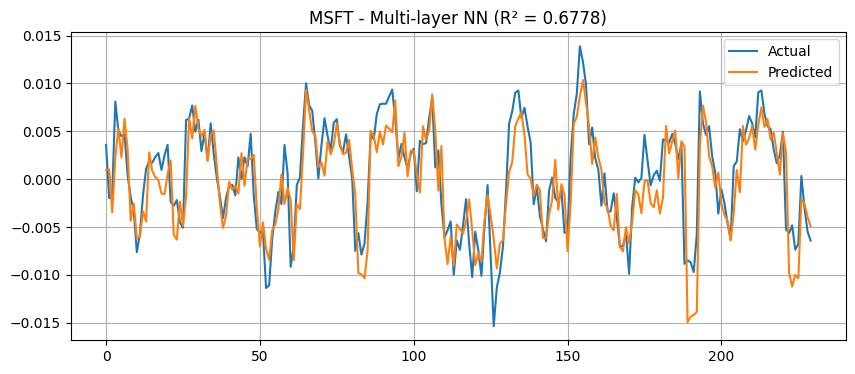
\includegraphics[width=0.85\textwidth]{MSFT_multi_layer_nn.png}

  \item \textbf{XOM}: Smoother but accurate predictions, although high-frequency deviations remain. $R^2 = 0.6257$.
  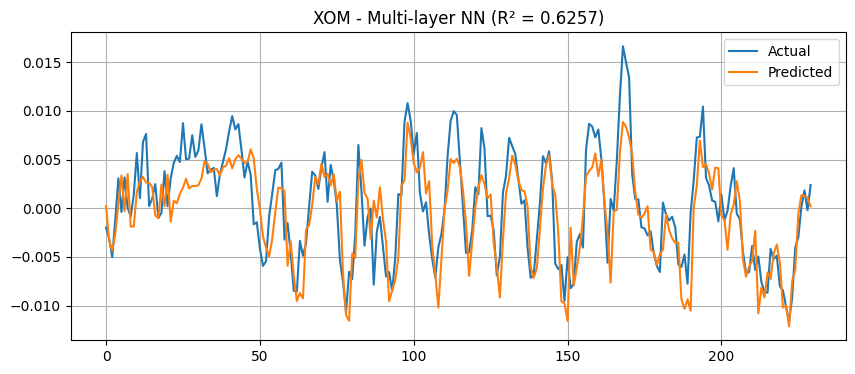
\includegraphics[width=0.85\textwidth]{XOM_multi_layer_nn.png}
\end{itemize}

\subsection{Summary of Results}
\begin{table}[h!]
\centering
\begin{tabular}{lccc}
\toprule
\textbf{Stock} & \textbf{MSE} & \textbf{RMSE} & \textbf{R$^2$} \\
\midrule
AAPL & 0.000015 & 0.003825 & 0.6270 \\
MSFT & 0.000010 & 0.003084 & 0.6778 \\
JPM  & 0.000025 & 0.004982 & 0.3381 \\
BAC  & 0.000010 & 0.003213 & 0.7554 \\
XOM  & 0.000011 & 0.003315 & 0.6257 \\
CVX  & 0.000011 & 0.003311 & 0.6768 \\
\bottomrule
\end{tabular}
\caption{Multi-Layer Neural Network Performance}
\end{table}

While some stocks such as JPM underperformed, the multi-layer network offered improved generalization for BAC, MSFT, and CVX. This confirms that deeper architectures can learn better representations—provided the underlying signal-to-noise ratio is favorable.

Daily stock returns remain notoriously hard to predict due to market randomness, but even moderate increases in $R^2$ can provide useful trading signals.
\section{Comparison: Single-Layer vs Multi-Layer Neural Networks}

In this section, we compare the performance of the single-layer and multi-layer neural network models across the six selected stocks. The goal is to understand the trade-offs in accuracy, generalization, and model complexity.

\subsection{Quantitative Performance Summary}
\begin{table}[h!]
\centering
\begin{tabular}{lcccccc}
\toprule
\textbf{Stock} & \multicolumn{3}{c}{\textbf{Single-Layer}} & \multicolumn{3}{c}{\textbf{Multi-Layer}} \\
\cmidrule(lr){2-4} \cmidrule(lr){5-7}
 & MSE & RMSE & R$^2$ & MSE & RMSE & R$^2$ \\
\midrule
AAPL & 0.000027 & 0.00518 & 0.6110 & 0.000015 & 0.00383 & 0.6270 \\
MSFT & 0.000020 & 0.00452 & 0.5868 & 0.000010 & 0.00308 & 0.6778 \\
JPM  & 0.000034 & 0.00584 & 0.4575 & 0.000025 & 0.00498 & 0.3381 \\
BAC  & 0.000024 & 0.00490 & 0.6703 & 0.000010 & 0.00321 & 0.7554 \\
XOM  & 0.000016 & 0.00405 & 0.6776 & 0.000011 & 0.00332 & 0.6257 \\
CVX  & 0.000017 & 0.00416 & 0.6990 & 0.000011 & 0.00331 & 0.6768 \\
\bottomrule
\end{tabular}
\caption{Performance Comparison: Single vs Multi-Layer Neural Networks}
\end{table}

\subsection{Model Behavior and Insights}
\textbf{Overall Improvement:} Across most stocks, the multi-layer model consistently achieved lower MSE and RMSE values and higher $R^2$ scores compared to the single-layer counterpart. This is expected as deeper networks capture non-linear patterns better.

\textbf{Best Performers:} BAC and MSFT stand out in the multi-layer setup with $R^2$ values exceeding 0.75 and 0.67 respectively, up from already decent baselines. These stocks may exhibit smoother trends and stronger signal-to-feature relationships.

\textbf{JPM Exception:} Unlike others, JPM showed reduced performance with the deeper model ($R^2$ dropped from 0.4575 to 0.3381). This suggests that either the additional layers overfit noise or failed to extract useful patterns. Financials may carry unpredictable or lagged responses to market information.

\textbf{Complexity vs Simplicity:} The single-layer model, though linear, performed surprisingly well for stocks like CVX and XOM. This shows that in certain contexts, simpler models can approximate returns effectively without risk of overfitting.

\subsection{Trade-Off Analysis}
\begin{itemize}
  \item \textbf{Accuracy:} Multi-layer networks outperform on most metrics but not universally. The marginal gains are most valuable when $R^2$ rises significantly (e.g., BAC, MSFT).
  \item \textbf{Robustness:} Single-layer networks are less prone to overfitting due to lower capacity. They performed relatively consistently across all stocks.
  \item \textbf{Interpretability:} Linear models offer more transparent behavior, aiding financial interpretability, which is often desirable in regulated environments.
  \item \textbf{Computation:} Multi-layer models require more resources and time, both in training and hyperparameter tuning.
\end{itemize}

\subsection{Conclusion of Comparison}
While the multi-layer model improves predictive performance across most stocks, its effectiveness is not uniform. Stock-specific volatility, noise, and nonlinearities play a significant role. Therefore, model selection in stock forecasting must balance complexity with generalizability.

In practice, a hybrid ensemble approach—or sector-specific model design—might yield the best results, leveraging strengths of both architectures based on the data characteristics.

\section{Conclusion}

This project investigated the viability of using feedforward neural networks to forecast next-day stock returns across multiple sectors—Technology, Finance, and Energy. We implemented two architectures: a simple single-layer neural network and a more expressive multi-layer neural network with hidden layers and nonlinear activations. Each model was evaluated on six prominent stocks (AAPL, MSFT, JPM, BAC, XOM, CVX) using regression metrics such as MSE, RMSE, and $R^2$.

Through detailed preprocessing and feature engineering, we incorporated technical indicators like lagged returns, moving averages, and volatility into our model inputs. The results showed that while both models capture some predictive patterns, multi-layer networks typically outperform single-layer ones, particularly for stocks with less erratic behavior. Nevertheless, the performance was stock-dependent—JPM, for instance, suffered from reduced performance in the deeper model, highlighting the non-trivial challenge of generalization in financial time series.

Importantly, even the best $R^2$ scores in this project hovered around 0.75. This underscores the inherent difficulty of stock prediction: markets are noisy, dynamic, and prone to sudden changes. Despite this, the fact that neural networks—especially multi-layer ones—can extract structure from such data is promising. Our findings suggest that while no single model is universally optimal, neural networks can be a valuable tool in a broader predictive analytics pipeline.

Future work could explore more sophisticated architectures like LSTMs or Transformers, incorporate macroeconomic indicators, and utilize ensemble approaches to balance variance and bias. Another promising direction is the integration of sentiment analysis and natural language processing (NLP). Since stock prices are often influenced by investor emotions and public sentiment—especially in reaction to breaking news, earnings announcements, or social media trends—models that account for emotional and textual signals from news articles, Twitter feeds, and Reddit forums could add valuable predictive power. Additionally, incorporating alternative data sources such as Google Trends, options flow, and institutional sentiment could further enhance prediction robustness. The potential for improvement remains significant, especially with richer datasets and advanced regularization techniques.

\clearpage
\section*{Appendix: Full Feature Generation Script}

\subsection*{Code: 01\_data\_collection\_and\_cleaning.ipynb (Extended Version)}

\begin{lstlisting}[language=Python]
import pandas as pd  # For data manipulation and analysis
import os  # For file system operations like creating directories

def generate_features(df):
    """
    Generate technical indicators and features from raw price data.
    
    Parameters:
    -----------
    df : pandas.DataFrame
        Raw stock data with at least 'Close' price column
        
    Returns:
    --------
    pandas.DataFrame
        Processed dataframe with additional technical features
    """
    df = df.copy()
    df['Close'] = pd.to_numeric(df['Close'], errors='coerce')
    df['Return'] = df['Close'].pct_change(fill_method=None)
    df['Lag_1'] = df['Return'].shift(1)
    df['Lag_2'] = df['Return'].shift(2)
    df['SMA_5'] = df['Close'].rolling(window=5).mean()
    df['SMA_10'] = df['Close'].rolling(window=10).mean()
    df['Volatility'] = df['Return'].rolling(window=10).std()
    return df.dropna()

os.makedirs('../data/processed', exist_ok=True)
tickers = ['AAPL', 'MSFT', 'JPM', 'BAC', 'XOM', 'CVX']

for ticker in tickers:
    df = pd.read_csv(f'../data/raw/{ticker}_raw.csv', index_col=0, parse_dates=True)
    df.index.name = 'Date'
    processed = generate_features(df)
    processed.to_csv(f'../data/processed/{ticker}_processed.csv')
    print(f"{ticker} processed.")
\end{lstlisting}

\clearpage
\subsection*{Code: 02\_feature\_engineering.ipynb – Feature Generation}

\begin{lstlisting}[language=Python]
import pandas as pd  # For data manipulation and analysis
import os  # For file system operations like creating directories

def generate_features(df):
    """
    Generate technical indicators and features from raw price data.
    
    Parameters:
    -----------
    df : pandas.DataFrame
        Raw stock data with at least 'Close' price column
        
    Returns:
    --------
    pandas.DataFrame
        Processed dataframe with additional technical features
    """
    df = df.copy()
    df['Close'] = pd.to_numeric(df['Close'], errors='coerce')
    df['Return'] = df['Close'].pct_change(fill_method=None)
    df['Lag_1'] = df['Return'].shift(1)
    df['Lag_2'] = df['Return'].shift(2)
    df['SMA_5'] = df['Close'].rolling(window=5).mean()
    df['SMA_10'] = df['Close'].rolling(window=10).mean()
    df['Volatility'] = df['Return'].rolling(window=10).std()
    return df.dropna()

os.makedirs('../data/processed', exist_ok=True)
tickers = ['AAPL', 'MSFT', 'JPM', 'BAC', 'XOM', 'CVX']

for ticker in tickers:
    df = pd.read_csv(f'../data/raw/{ticker}_raw.csv', index_col=0, parse_dates=True)
    df.index.name = 'Date'
    processed = generate_features(df)
    processed.to_csv(f'../data/processed/{ticker}_processed.csv')
    print(f"{ticker} processed.")
\end{lstlisting}

\subsection*{Code: 02\_feature\_engineering.ipynb – DataFrame Analysis}

\begin{lstlisting}[language=Python]
import pandas as pd
import matplotlib.pyplot as plt
import os
import seaborn as sns

tickers = ['AAPL', 'MSFT', 'JPM', 'BAC', 'XOM', 'CVX']
processed_dfs = {}

for ticker in tickers:
    file_path = f'../data/processed/{ticker}_processed.csv'
    processed_dfs[ticker] = pd.read_csv(file_path, index_col='Date', parse_dates=True)
    print(f"Loaded {ticker} data with {processed_dfs[ticker].shape[0]} rows and {processed_dfs[ticker].shape[1]} columns")

print("\nApple (AAPL) processed data sample:")
print(processed_dfs['AAPL'].head())

print("\nApple (AAPL) summary statistics:")
print(processed_dfs['AAPL'].describe())

print("\nCorrelation between AAPL features:")
plt.figure(figsize=(12, 10))
sns.heatmap(processed_dfs['AAPL'].corr(), annot=True, cmap='coolwarm', fmt='.2f', linewidths=0.5)
plt.title('AAPL Feature Correlations')
plt.tight_layout()
plt.show()

plt.figure(figsize=(14, 7))
for ticker in tickers:
    normalized_price = processed_dfs[ticker]['Close'] / processed_dfs[ticker]['Close'].iloc[0] * 100
    plt.plot(processed_dfs[ticker].index, normalized_price, label=ticker)
plt.title('Normalized Stock Prices (Starting Price = 100)')
plt.xlabel('Date')
plt.ylabel('Normalized Price')
plt.legend()
plt.grid(True)
plt.show()

plt.figure(figsize=(14, 7))
for ticker in tickers:
    plt.plot(processed_dfs[ticker].index, processed_dfs[ticker]['Volatility'], label=f"{ticker} Volatility")
plt.title('Volatility Comparison Across Stocks')
plt.xlabel('Date')
plt.ylabel('Volatility (10-day rolling std)')
plt.legend()
plt.grid(True)
plt.show()

tech_stocks = ['AAPL', 'MSFT']
finance_stocks = ['JPM', 'BAC']
energy_stocks = ['XOM', 'CVX']

sectors = {
    'Technology': tech_stocks,
    'Finance': finance_stocks,
    'Energy': energy_stocks
}

sector_stats = pd.DataFrame()

for sector_name, sector_tickers in sectors.items():
    sector_returns = pd.concat([processed_dfs[ticker]['Return'] for ticker in sector_tickers], axis=1)
    sector_stats[f'{sector_name}_Avg_Return'] = sector_returns.mean(axis=1)
    
    sector_volatility = pd.concat([processed_dfs[ticker]['Volatility'] for ticker in sector_tickers], axis=1)
    sector_stats[f'{sector_name}_Avg_Volatility'] = sector_volatility.mean(axis=1)

print("\nSector average statistics:")
print(sector_stats.describe())

plt.figure(figsize=(14, 7))
for sector in sectors.keys():
    plt.plot(sector_stats.index, sector_stats[f'{sector}_Avg_Return'], label=f"{sector} Avg Return")
plt.title('Average Returns by Sector')
plt.xlabel('Date')
plt.ylabel('Average Return')
plt.legend()
plt.grid(True)
plt.show()
\end{lstlisting}
\clearpage
\subsection*{Code: 03\_modeling\_single\_layer\_nn.py – Full Modeling Script (Single-Layer NN)}

\begin{lstlisting}[language=Python]
import sys
sys.path.append('..') # Add parent directory to Python path to import modules from parent directory
import json # For saving feature names to JSON files
import pandas as pd # For data manipulation and analysis
import numpy as np # For numerical operations
import os # For file system operations
import random # For setting random seed
import tensorflow as tf # Deep learning framework
from sklearn.model_selection import train_test_split # For splitting data into train and test sets
from sklearn.preprocessing import StandardScaler # For standardizing features to zero mean and unit variance
from sklearn.feature_selection import mutual_info_regression # For feature selection using information theory
from sklearn.metrics import mean_squared_error, r2_score # For model evaluation
import matplotlib.pyplot as plt # For data visualization
from tensorflow.keras.models import Sequential # For creating sequential neural network models
from tensorflow.keras.layers import Dense # For creating fully connected neural network layers
from tensorflow.keras.callbacks import EarlyStopping, ReduceLROnPlateau # For optimizing training process
import logging # For controlling log output

# Suppress TensorFlow warnings to keep notebook output clean
# Level 2 hides info and warnings but shows errors
os.environ['TF_CPP_MIN_LOG_LEVEL'] = '2'
logging.getLogger('tensorflow').setLevel(logging.ERROR)

# Set random seeds for reproducibility across runs
# This ensures that random operations like weight initialization and train/test splits are consistent
np.random.seed(42)
tf.random.set_seed(42)
random.seed(42)

# List of stock tickers representing different market sectors
# AAPL, MSFT: Technology
# JPM, BAC: Banking/Finance
# XOM, CVX: Energy/Oil
tickers = ['AAPL', 'MSFT', 'JPM', 'BAC', 'XOM', 'CVX']
results = {} # Dictionary to store performance metrics for each ticker

# Iterate through each ticker to build individual models
for ticker in tickers:
    print(f"Training {ticker}...")
    # Load processed price data for current ticker
    # Parse_dates ensures that the date index is properly formatted
    df = pd.read_csv(f'../data/processed/{ticker}_processed.csv', index_col='Date', parse_dates=True)
    df['Close'] = pd.to_numeric(df['Close'], errors='coerce') # Convert 'Close' column to numeric, handling any errors

    # ------ Feature Engineering: Technical Indicators ------
    # Calculate daily percentage change in closing price
    df['Return'] = df['Close'].pct_change()
    
    # Create lagged returns (previous 1-5 days) to capture short-term price patterns
    # These features help the model understand recent market momentum
    for i in range(1, 6):
        df[f'Lag_{i}'] = df['Return'].shift(i)
    
    # 10-day price momentum: difference between current price and price 10 days ago
    # Captures medium-term trend direction
    df['Momentum_10'] = df['Close'] - df['Close'].shift(10)

    # Calculate RSI (Relative Strength Index) - popular technical indicator
    # RSI measures the magnitude of recent price changes to evaluate overbought/oversold conditions
    delta = df['Close'].diff() # Daily price difference
    gain = delta.clip(lower=0).rolling(14).mean() # Average gains over 14 days (standard RSI period)
    loss = -delta.clip(upper=0).rolling(14).mean() # Average losses over 14 days
    rs = gain / (loss.replace(0, np.finfo(float).eps)) # Relative strength (gain/loss ratio), avoiding division by zero
    df['RSI'] = 100 - (100 / (1 + rs)) # RSI formula: scales result to 0-100 range

    # Calculate MACD (Moving Average Convergence Divergence)
    # MACD is a trend-following momentum indicator showing relationship between two moving averages
    ema12 = df['Close'].ewm(span=12, adjust=False).mean() # 12-day exponential moving average
    ema26 = df['Close'].ewm(span=26, adjust=False).mean() # 26-day exponential moving average
    df['MACD'] = ema12 - ema26 # MACD line is difference between these EMAs
    df['MACD_signal'] = df['MACD'].ewm(span=9, adjust=False).mean() # 9-day EMA of MACD (signal line)

    # ------ Target Variable Creation ------
    # Log returns are preferred in finance as they're additive over time and more normally distributed
    df['LogReturn'] = np.log(df['Close'] / df['Close'].shift(1))
    # Target: 3-day smoothed forward log return
    # Shift(-1) looks one day ahead, rolling(3).mean() smooths over 3 days to reduce noise
    df['Target'] = df['LogReturn'].shift(-1).rolling(3).mean()

    # Remove rows with NaN values resulting from the lag and rolling operations
    df.dropna(inplace=True)

    # ------ Feature Selection using Mutual Information ------
    # Mutual information measures how much information one variable provides about another
    # It can capture non-linear relationships unlike correlation
    all_features = df.drop(columns=['Target']) # All columns except target
    target = df['Target']

    # Calculate mutual information between each feature and target
    mi_scores = mutual_info_regression(all_features, target)
    # Convert to Series, sort by MI score, and select top 10 most informative features
    top_features = pd.Series(mi_scores, index=all_features.columns).sort_values(ascending=False).head(10).index.tolist()

    # Create feature matrix X and target vector y using only selected features
    X = all_features[top_features]
    y = target

    # ------ Target Normalization ------
    # Normalize target to zero mean and unit standard deviation
    # This improves neural network training stability and convergence speed
    y_mean, y_std = y.mean(), y.std()
    y = (y - y_mean) / y_std

    # ------ Data Splitting ------
    # Split data chronologically (no shuffle) to maintain time-series integrity
    # Use 80% for training and 20% for testing
    X_train, X_test, y_train, y_test = train_test_split(X, y, shuffle=False, test_size=0.2)

    # ------ Feature Scaling ------
    # Standardize features to zero mean and unit variance
    # Neural networks perform better with standardized inputs
    scaler = StandardScaler()
    X_train_scaled = scaler.fit_transform(X_train) # Fit scaler on training data only to prevent data leakage
    X_test_scaled = scaler.transform(X_test) # Apply same transformation to test data

    # ------ Model Architecture ------
    # Create a single-layer neural network (linear model)
    # Single dense layer with one output neuron makes this equivalent to linear regression
    model = Sequential([
        Dense(1, input_shape=(X_train_scaled.shape[1],))
    ])
    model.compile(optimizer='adam', loss='mse') # Adam optimizer and mean squared error loss function

    # ------ Training Callbacks ------
    # Early stopping to prevent overfitting
    # Stops training when validation loss doesn't improve for 15 epochs
    early_stop = EarlyStopping(patience=15, restore_best_weights=True, monitor='val_loss')
    
    # Learning rate reduction
    # Reduces learning rate by half when validation loss plateaus for 5 epochs
    # Helps fine-tune model training when approaching optimal weights
    reduce_lr = ReduceLROnPlateau(monitor='val_loss', factor=0.5, patience=5, min_lr=1e-5, verbose=0)

    # ------ Model Training ------
    # Train for up to 200 epochs with 20% of training data used for validation
    # verbose=0 suppresses training output for cleaner notebook
    model.fit(X_train_scaled, y_train, validation_split=0.2, epochs=200, verbose=0,
              callbacks=[early_stop, reduce_lr])

    # ------ Save Model and Feature List ------
    # Create directory if it doesn't exist
    os.makedirs('../models/saved_model', exist_ok=True)
    # Save trained model in Keras format
    model.save(f'../models/saved_model/{ticker}_single_layer_nn.keras')
    # Save list of selected features for later use in prediction
    with open(f'../models/saved_model/{ticker}_single_layer_features.json', 'w') as f:
        json.dump(top_features, f)
    
    # ------ Generate Predictions ------
    # Make predictions on test set
    y_pred = model.predict(X_test_scaled, verbose=0).flatten() # Suppress prediction output
    
    # ------ De-normalize Predictions and Actual Values ------
    # Convert standardized values back to original scale for meaningful evaluation
    y_pred = y_pred * y_std + y_mean
    y_test_actual = y_test * y_std + y_mean

    # ------ Calculate Performance Metrics ------
    mse = mean_squared_error(y_test_actual, y_pred) # Mean Squared Error
    rmse = np.sqrt(mse) # Root Mean Squared Error - more interpretable in original units
    r2 = r2_score(y_test_actual, y_pred) # R-squared - proportion of variance explained by model
    results[ticker] = (mse, rmse, r2) # Store metrics for later comparison

    # ------ Visualize Results ------
    # Plot actual vs predicted values for visual assessment
    plt.figure(figsize=(10, 4))
    plt.plot(y_test_actual.values, label='Actual')
    plt.plot(y_pred, label='Predicted')
    plt.title(f"{ticker} - Single Layer NN (R² = {r2:.4f})")
    plt.legend()
    plt.grid(True)
    plt.show()

# ------ Summary Output ------
# Print performance metrics for all tickers for comparison
print("\nSUMMARY")
for ticker, (mse, rmse, r2) in results.items():
    print(f"{ticker}: MSE = {mse:.6f}, RMSE = {rmse:.6f}, R² = {r2:.4f}")
\end{lstlisting}
\clearpage
\subsection*{Code: 04\_modeling\_multi\_layer\_nn.ipynb – Full Modeling Script (Multi-Layer NN)}

\begin{lstlisting}[language=Python]
import pandas as pd # For data manipulation and analysis
import json # For saving feature lists
import numpy as np # For numerical operations
from sklearn.model_selection import train_test_split # For splitting data into train and test sets
from sklearn.preprocessing import StandardScaler, RobustScaler # For feature scaling
from tensorflow.keras.models import Sequential # For building neural network architecture
from tensorflow.keras.layers import Dense, Dropout, BatchNormalization # For network layers
from tensorflow.keras.callbacks import EarlyStopping, ReduceLROnPlateau, ModelCheckpoint # For optimizing training
from tensorflow.keras.regularizers import l2 # For adding regularization to reduce overfitting
from tensorflow.keras.optimizers import Adam # For adaptive learning rate optimization
from sklearn.metrics import mean_squared_error, r2_score # For model evaluation
import matplotlib.pyplot as plt # For visualizing results
import os # For file system operations
from sklearn.feature_selection import mutual_info_regression, SelectKBest # For information-based feature selection
import logging # For controlling log output

# Set random seeds for reproducibility across runs
# This ensures consistent results for weight initialization and data splitting
import random
import tensorflow as tf
np.random.seed(42)
tf.random.set_seed(42)
random.seed(42)

# Suppress TensorFlow warnings for cleaner output
os.environ['TF_CPP_MIN_LOG_LEVEL'] = '2'  # 0=all, 1=info, 2=warning, 3=error
logging.getLogger('tensorflow').setLevel(logging.ERROR)

# Define stock tickers from different market sectors for analysis
tickers = ['AAPL', 'MSFT', 'JPM', 'BAC', 'XOM', 'CVX']
results = {} # Dictionary to store evaluation metrics for each ticker

# Process each ticker individually with its own model
for ticker in tickers:
    print(f"\nTraining {ticker}...")
    # Load processed price data from CSV with dates as index
    df = pd.read_csv(f'../data/processed/{ticker}_processed.csv', index_col='Date', parse_dates=True)
    df['Close'] = pd.to_numeric(df['Close'], errors='coerce') # Ensure Close prices are numeric

    # === Enhanced Feature Engineering ===
    # Basic price-based features: returns and transformations
    df['Return'] = df['Close'].pct_change() # Daily percentage change in price
    df['Return_Abs'] = np.abs(df['Return']) # Magnitude of price changes (volatility indicator)
    df['Log_Return'] = np.log(df['Close'] / df['Close'].shift(1)) # Log returns for statistical properties
    
    # Return lags - capture autocorrelation patterns in price movements
    # Using up to 9 days of history to identify recurring patterns
    for i in range(1, 10):
        df[f'Lag_{i}'] = df['Return'].shift(i) # Past returns as predictors
        if i <= 5:  # Create non-linear transformations for recent days
            df[f'Lag_{i}_squared'] = df[f'Lag_{i}']**2 # Squared terms capture magnitude effects
            
    # Momentum indicators at different timeframes
    # Price differences across various windows to identify trends
    for window in [5, 10, 20, 30]:
        df[f'Momentum_{window}'] = df['Close'] - df['Close'].shift(window) # Absolute change
        df[f'Momentum_Ratio_{window}'] = df['Close'] / df['Close'].shift(window) # Relative change
    
    # Moving averages - common smoothing technique in technical analysis
    # Longer windows identify longer-term trends
    for window in [5, 10, 20, 50, 100]:
        df[f'MA_{window}'] = df['Close'].rolling(window=window).mean() # Simple moving average
        # Distance between current price and moving average (normalized)
        df[f'Close_MA_{window}_Ratio'] = df['Close'] / df[f'MA_{window}'] # Relative position to trend
    
    # Volatility features at different timeframes
    # Standard deviation of returns measures price variability
    for window in [5, 10, 20, 30]:
        df[f'Volatility_{window}'] = df['Return'].rolling(window=window).std() # Historical volatility
        # Normalize short-term volatility relative to recent volatility trend
        if window in [5, 10]:
            df[f'Volatility_Ratio_{window}'] = df[f'Volatility_{window}'] / df[f'Volatility_{window}'].rolling(window=5).mean()
    
    # RSI (Relative Strength Index) at multiple timeframes
    # Momentum oscillator measuring speed and change of price movements
    for window in [6, 14, 21]: # 14 is standard, also include shorter and longer periods
        delta = df['Close'].diff() # Daily price changes
        gain = delta.clip(lower=0).rolling(window).mean() # Average gains over period
        loss = -delta.clip(upper=0).rolling(window).mean() # Average losses over period
        rs = gain / (loss.replace(0, np.finfo(float).eps)) # Relative strength ratio
        df[f'RSI_{window}'] = 100 - (100 / (1 + rs)) # RSI formula (0-100 scale)
    
    # MACD (Moving Average Convergence Divergence) - trend-following momentum indicator
    # Shows relationship between two moving averages of price
    ema12 = df['Close'].ewm(span=12, adjust=False).mean() # 12-day exponential moving average
    ema26 = df['Close'].ewm(span=26, adjust=False).mean() # 26-day exponential moving average
    df['MACD'] = ema12 - ema26 # MACD line
    df['MACD_signal'] = df['MACD'].ewm(span=9, adjust=False).mean() # 9-day EMA of MACD
    df['MACD_hist'] = df['MACD'] - df['MACD_signal'] # Histogram (difference between MACD and signal line)
    df['MACD_hist_diff'] = df['MACD_hist'].diff() # Change in histogram (acceleration/deceleration)
    
    # Bollinger Bands - volatility bands placed above and below moving average
    # Wider bands indicate higher volatility, narrower bands indicate lower volatility
    for window in [20]: # 20 is standard period
        middle_band = df['Close'].rolling(window=window).mean() # Center band (20-day SMA)
        std_dev = df['Close'].rolling(window=window).std() # Standard deviation of price
        df[f'BB_upper_{window}'] = middle_band + (std_dev * 2) # Upper band (2 std devs above)
        df[f'BB_lower_{window}'] = middle_band - (std_dev * 2) # Lower band (2 std devs below)
        df[f'BB_width_{window}'] = (df[f'BB_upper_{window}'] - df[f'BB_lower_{window}']) / middle_band # Band width (volatility)
        df[f'BB_position_{window}'] = (df['Close'] - df[f'BB_lower_{window}']) / (df[f'BB_upper_{window}'] - df[f'BB_lower_{window}']) # Position within bands
    
    # Rate of Change - percentage change in price over specified periods
    # Measures momentum by comparing current price to price n periods ago
    for window in [5, 10, 21]:
        df[f'ROC_{window}'] = df['Close'].pct_change(window) * 100 # Expressed as percentage
    
    # Volume features (if available) - provide insight into strength of price movements
    if 'Volume' in df.columns:
        df['Volume'] = pd.to_numeric(df['Volume'], errors='coerce')
        df['Log_Volume'] = np.log(df['Volume'] + 1) # Log transformation for statistical properties
        df['Volume_Change'] = df['Volume'].pct_change() # Day-over-day volume change
        
        # Volume moving averages - identify abnormal volume levels
        for window in [5, 10, 20]:
            df[f'Volume_SMA_{window}'] = df['Volume'].rolling(window).mean()
            df[f'Volume_Ratio_{window}'] = df['Volume'] / df[f'Volume_SMA_{window}'] # Current volume relative to average
        
        # Price-volume relationships - volume often confirms price movements
        df['Volume_Return_Ratio'] = df['Volume'] / (df['Return_Abs'] + 0.001) # Avoid division by zero
        df['Volume_Close_Ratio'] = df['Volume'] / df['Close'] # Volume relative to price level

    # Define target variable: 5-day smoothed forward log return
    # Using 5-day smoothing reduces noise in the prediction target
    df['LogReturn'] = np.log(df['Close'] / df['Close'].shift(1))
    df['Target'] = df['LogReturn'].shift(-1).rolling(5).mean() # Looking ahead 1 day, smoothing over 5 days

    # Remove rows with NaN values from lag operations and rolling windows
    df = df.dropna()
    
    # Handle outliers by clipping extreme values
    # This prevents rare events from dominating model training
    for col in df.columns:
        if col != 'Close' and col != 'Target':  # Preserve original price and target
            lower_bound = df[col].quantile(0.005) # 0.5% percentile
            upper_bound = df[col].quantile(0.995) # 99.5% percentile
            df[col] = df[col].clip(lower=lower_bound, upper=upper_bound) # Trim outliers
        # Feature selection using mutual information
    # This measures the non-linear relationship between each feature and target
    if df.shape[1] > 30:  # Only perform selection if we have many features
        X_temp = df.drop(columns=['Close', 'Target', 'LogReturn', 'Return']) # Candidate features
        y_temp = df['Target'] # Target variable
        
        # Calculate mutual information between each feature and target
        mi_scores = mutual_info_regression(X_temp, y_temp)
        mi_df = pd.DataFrame({'Feature': X_temp.columns, 'MI_Score': mi_scores})
        mi_df = mi_df.sort_values('MI_Score', ascending=False) # Rank features by information content
        
        # Select top 25 features plus essential technical indicators
        top_features = mi_df.head(25)['Feature'].tolist() # Top 25 by mutual information
        essential_features = [col for col in X_temp.columns if 'RSI' in col or 'MACD' in col 
                               or 'Momentum' in col or 'Volatility' in col] # Key technical indicators
        selected_features = list(set(top_features + essential_features)) # Combine lists, remove duplicates
        
        # Create feature matrix with only selected features
        X = df[selected_features]
    else:
        # If few features, just drop redundant ones
        X = df.drop(columns=['Return', 'Close', 'Target', 'LogReturn', 'Log_Return'])
    
    # Define target vector
    y = df['Target']

    # Normalize target variable to improve model convergence
    y_mean, y_std = y.mean(), y.std() # Calculate statistics
    # Split chronologically without shuffling to preserve time-series nature
    y_train, y_test = train_test_split(y, shuffle=False, test_size=0.2) 
    y_train_norm = (y_train - y_mean) / y_std # Standardize training targets
    y_test_norm = (y_test - y_mean) / y_std # Standardize test targets using same parameters

    # Split features chronologically (train-test split)
    X_train, X_test = train_test_split(X, shuffle=False, test_size=0.2)

    # Scale features with RobustScaler which is less influenced by outliers than StandardScaler
    scaler = RobustScaler()  # Uses median and interquartile range instead of mean and variance
    X_train_scaled = scaler.fit_transform(X_train) # Fit on training data only
    X_test_scaled = scaler.transform(X_test) # Apply same transformation to test data
    
    # === Build a deep neural network with regularization ===
    # Architecture designed to balance complexity, overfitting prevention, and learning capacity
    
    model = Sequential([
        # First layer - largest to capture complex patterns
        Dense(192, activation='relu', input_shape=(X_train_scaled.shape[1],), 
              kernel_regularizer=l2(0.0001)), # L2 regularization prevents large weights
        BatchNormalization(), # Normalizes layer inputs for more stable training
        Dropout(0.3), # Randomly drops 30% of neurons during training to prevent overfitting
        
        # Second layer - halve the neurons
        Dense(96, activation='relu', kernel_regularizer=l2(0.0001)), 
        BatchNormalization(),
        Dropout(0.2), # Gradually decrease dropout rate in deeper layers
        
        # Third layer - further reduction in complexity
        Dense(48, activation='relu', kernel_regularizer=l2(0.0001)), 
        BatchNormalization(),
        Dropout(0.2),

        # Fourth layer - final hidden layer for fine-tuning
        Dense(24, activation='relu', kernel_regularizer=l2(0.0001)), 
        BatchNormalization(),
        Dropout(0.1),
        
        # Output layer - single neuron for regression prediction
        Dense(1) # No activation function for unbounded regression output
    ])
    
    # Compile with Adam optimizer - adaptive learning rate method
    optimizer = Adam(learning_rate=0.001) # Initial learning rate
    model.compile(optimizer=optimizer, loss='mse') # Mean squared error loss for regression

    # === Training Strategy with Advanced Callbacks ===
    
    # Create a weight folder for this ticker to save checkpoints
    model_folder = f'../models/saved_model/{ticker}_weights'
    os.makedirs(model_folder, exist_ok=True)
    
    # Model checkpoint to save the best model during training
    checkpoint = ModelCheckpoint(
        filepath=f'{model_folder}/best_checkpoint_v4.keras', # Use .keras format instead of .h5
        monitor='val_loss', # Track validation loss
        save_best_only=True, # Only save when model improves
        mode='min', # Lower validation loss is better
        verbose=0  # Suppress output messages
    )
    
    # Early stopping to prevent overfitting
    # Stops training when validation loss stops improving
    early_stop = EarlyStopping(
        monitor='val_loss',
        patience=25, # Wait 25 epochs before stopping
        restore_best_weights=True, # Restore weights from epoch with best validation loss
        mode='min',
        verbose=0  # Suppress output messages
    )
    
    # Learning rate reduction when training plateaus
    # Reduces learning rate when validation loss stops improving
    reduce_lr = ReduceLROnPlateau(
        monitor='val_loss',
        factor=0.5,  # Multiply learning rate by 0.5 when triggered
        patience=8,  # Wait 8 epochs before reducing
        min_lr=1e-6, # Minimum learning rate
        mode='min',
        verbose=0  # Suppress output messages
    )
    
    # Train model with validation split for monitoring
    print(f"Training {ticker} model...")
    history = model.fit(
        X_train_scaled, y_train_norm, # Training data
        validation_split=0.2, # Use 20% of training data for validation
        epochs=100, # Maximum number of epochs
        batch_size=64, # Process 64 samples per gradient update
        verbose=0, # Suppress epoch-by-epoch output
        callbacks=[early_stop, reduce_lr, checkpoint] # Use all three callbacks
    )

    # Save final model and selected features
    os.makedirs('../models/saved_model', exist_ok=True)
    model.save(f'../models/saved_model/{ticker}_multi_layer_nn.keras') # Use .keras format
    with open(f'../models/saved_model/{ticker}_multi_layer_features.json', 'w') as f:
        json.dump(selected_features, f)  # Save feature names for later use
        
    # === Generate predictions and evaluate model performance ===
    y_pred_norm = model.predict(X_test_scaled, verbose=0).flatten()  # Suppress prediction output
    # Convert standardized predictions back to original scale
    y_pred = y_pred_norm * y_std + y_mean # De-normalize predictions
    y_test_actual = y_test.values # Actual values for comparison

    # Calculate performance metrics
    mse = mean_squared_error(y_test_actual, y_pred) # Mean Squared Error
    rmse = np.sqrt(mse)  # Root Mean Squared Error (in original units)
    r2 = r2_score(y_test_actual, y_pred) # R-squared (proportion of variance explained)
    results[ticker] = (mse, rmse, r2)  # Store metrics for comparison

    # Visualize predictions vs actual values
    plt.figure(figsize=(10, 4))
    plt.plot(y_test_actual, label='Actual')
    plt.plot(y_pred, label='Predicted')
    plt.title(f"{ticker} - Multi-layer NN (R² = {r2:.4f})")
    plt.legend()
    plt.grid(True)
    plt.show()

# Print summary of results for all tickers
print("\nSUMMARY OF MULTI-LAYER NN MODEL")
for ticker, (mse, rmse, r2) in results.items():
    print(f"{ticker}: MSE = {mse:.6f}, RMSE = {rmse:.6f}, R² = {r2:.4f}")
\end{lstlisting}
